% Figure 1 — the four limitations this work answers.
% Standalone: pdflatex fig_problem_solution.tex.  txfonts matches the body.
\documentclass[border=3pt]{standalone}
\usepackage[T1]{fontenc}
\usepackage{amsmath}
\usepackage{txfonts}
\usepackage{tikz}
\usetikzlibrary{positioning, arrows.meta, calc}

\definecolor{fink}{HTML}{1E2E3A}
\definecolor{teal}{HTML}{2F6F68}
\definecolor{slate2}{HTML}{E4EBF1}
\definecolor{sandF}{HTML}{F2EAE0}
\definecolor{sandL}{HTML}{7A6F5F}
\definecolor{brassF}{HTML}{EFDCC6}
\definecolor{brassL}{HTML}{A8763A}

\tikzset{
  thin/.style     = {line width=0.4pt},
  form/.style     = {line width=0.9pt, rounded corners=0pt},
  axis/.style     = {->, >={Stealth[length=1.2mm]}, line width=0.5pt, fink!70},
  flowthin/.style = {->, >={Stealth[length=1.5mm]}, line width=0.9pt, fink!85},
  flow/.style     = {->, >={Stealth[length=2.6mm]}, line width=1.6pt, brassL},
  dim/.style      = {<->, >={Stealth[length=1.2mm]}, line width=0.5pt, brassL},
  rule/.style     = {line width=0.5pt, black!55},
  lab/.style      = {font=\scriptsize, text=fink, align=left},
  val/.style      = {font=\scriptsize, text=fink},
  note/.style     = {font=\tiny, text=fink!78, align=center},
}

\begin{document}
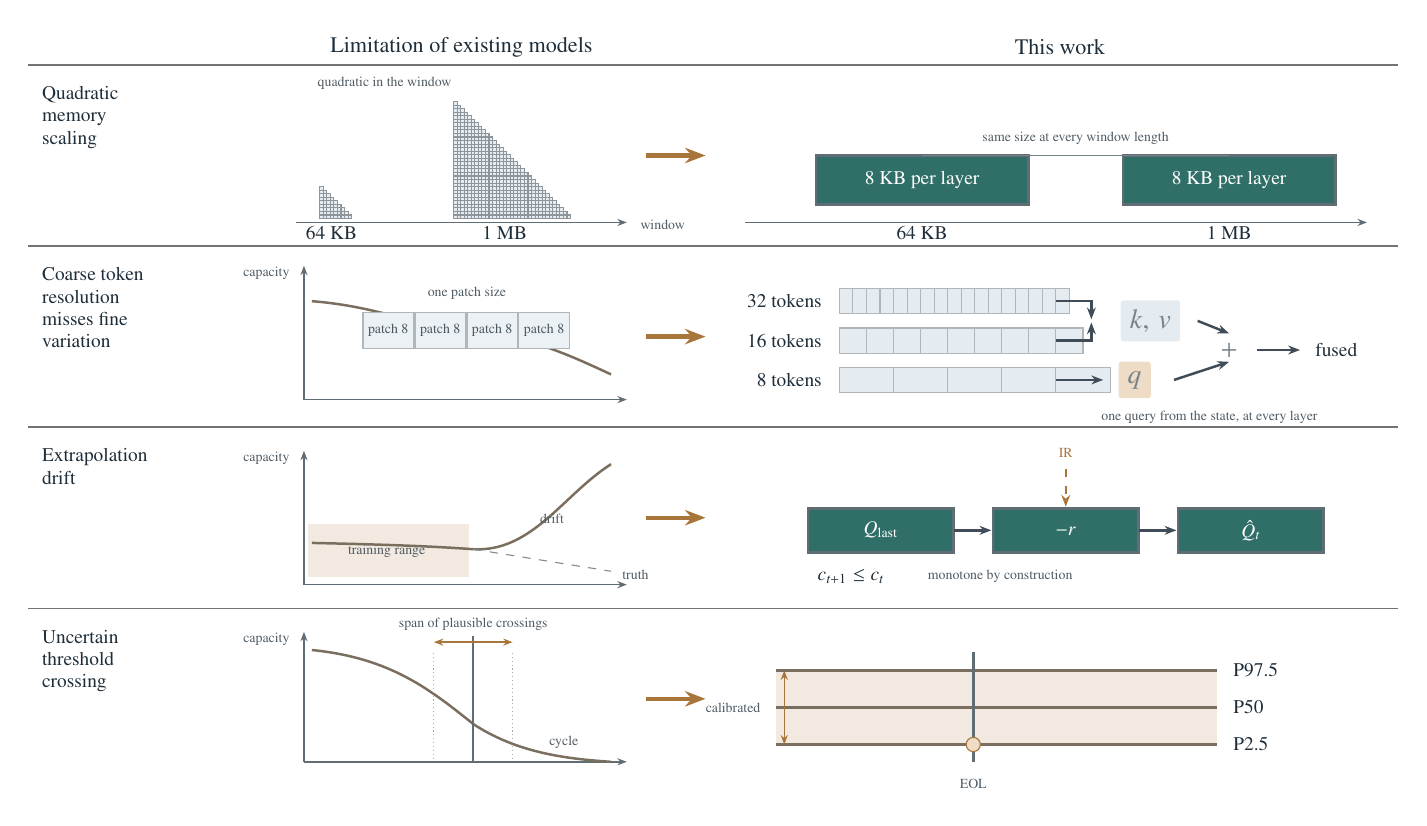
\begin{tikzpicture}

% grid: label 0.35 | problem 3.6-8.0 | arrow 8.15-8.85 | solution 9.2-17.7
% rows: 10.55 | 8.25 | 5.95 | 3.65

\node[font=\footnotesize, text=fink] at (5.80,10.78) {Limitation of existing models};
\node[font=\footnotesize, text=fink] at (13.40,10.78) {This work};
\foreach \y in {10.55,8.25,5.95,3.65}{\draw[rule] (0.30,\y) -- (17.70,\y);}
\foreach \y in {9.40,7.10,4.80,2.50}{\draw[flow] (8.15,\y) -- (8.90,\y);}

% ================================================================= row 1
\node[lab, anchor=north west] at (0.35,10.40) {Quadratic\\memory\\scaling};

% problem: a causal mask grows with the window
\foreach \n/\x in {8/4.00, 32/5.70}{
  \foreach \r in {0,...,\n}{
    \pgfmathsetmacro{\ry}{\n-\r}
    \foreach \c in {0,...,\r}{
      \draw[thin, fink!50, fill=slate2] (\x+\c*0.045,8.60+\ry*0.045) rectangle ++(0.045,0.045);
    }}}
\draw[axis] (3.70,8.55) -- (7.90,8.55);
\node[val] at (4.15,8.42) {64 KB};
\node[val] at (6.35,8.42) {1 MB};
\node[note, anchor=west] at (7.95,8.52) {window};
\node[note, anchor=west] at (3.85,10.32) {quadratic in the window};

% answer: the state is the same size at both windows
\draw[axis] (9.40,8.55) -- (17.30,8.55);
\foreach \x in {10.30,14.20}{
  \draw[form, fink!70, fill=teal] (\x,8.78) rectangle ++(2.70,0.62);
  \node[font=\scriptsize, text=white] at (\x+1.35,9.09) {8 KB per layer};
}
\draw[thin, fink!60] (11.65,9.40) -- (15.55,9.40);
\node[note, anchor=south] at (13.60,9.42) {same size at every window length};
\node[val] at (11.65,8.42) {64 KB};
\node[val] at (15.55,8.42) {1 MB};

% ================================================================= row 2
\node[lab, anchor=north west] at (0.35,8.10) {Coarse token\\resolution\\misses fine\\variation};

% problem: one coarse tiling over a segment that contains a dip
\draw[axis] (3.80,6.30) -- (7.90,6.30);
\draw[axis] (3.80,6.30) -- (3.80,8.00);
\node[note, anchor=east] at (3.74,7.90) {capacity};
\draw[form, sandL] (3.90,7.55) .. controls (4.80,7.48) and (5.30,7.20) .. (5.90,7.16)
                    .. controls (6.60,7.12) and (7.10,6.90) .. (7.70,6.62);
\foreach \k in {0,1,2,3}{
  \draw[thin, fink!35, fill=slate2!70] (4.55+\k*0.66,6.95) rectangle ++(0.64,0.46);
  \node[font=\tiny, text=fink!80] at (4.87+\k*0.66,7.18) {patch 8};
}
\node[note, anchor=south] at (5.87,7.45) {one patch size};

% answer: three tilings of the same segment, coarse state becomes the query
\foreach \lab/\n/\y in {32 tokens/16/7.55, 16 tokens/8/7.05, 8 tokens/4/6.55}{
  \pgfmathsetmacro{\tw}{2.75/\n}
  \foreach \k in {0,...,\n}{
    \draw[thin, fink!35, fill=slate2] (10.60+\k*\tw,\y-0.16) rectangle ++(\tw,0.32);
  }
  \node[val, anchor=east] at (10.50,\y) {\lab};
}
% the fusion itself: the coarse state becomes the query, the other two
% branches supply keys and values, and the result is written back
\draw[flowthin] (13.35,7.55) -- (13.80,7.55) -- (13.80,7.32);
\draw[flowthin] (13.35,7.05) -- (13.80,7.05) -- (13.80,7.28);
\node[form, fink!60, fill=slate2, rounded corners=1pt] (kv) at (14.55,7.30) {$k,\,v$};
\draw[flowthin] (13.35,6.55) -- (13.95,6.55);
\node[form, fink!60, fill=brassF, rounded corners=1pt] (q) at (14.35,6.55) {$q$};
\node[form, circle, fink!60, fill=white, minimum size=4.6mm, inner sep=0pt] (add) at (15.55,6.93) {$+$};
\draw[flowthin] (15.15,7.30) -- (15.55,7.14);
\draw[flowthin] (14.85,6.55) -- (15.55,6.78);
\draw[flowthin] (15.90,6.93) -- (16.45,6.93);
\node[val, anchor=west] at (16.52,6.93) {fused};
\node[note, anchor=north] at (15.30,6.28) {one query from the state, at every layer};

% ================================================================= row 3
\node[lab, anchor=north west] at (0.35,5.80) {Extrapolation\\drift};

% problem: a data-driven model leaves its training range
\draw[axis] (3.80,3.95) -- (7.90,3.95);
\draw[axis] (3.80,3.95) -- (3.80,5.65);
\node[note, anchor=east] at (3.74,5.55) {capacity};
\draw[fill=sandF, draw=none] (3.85,4.05) rectangle (5.90,4.72);
\node[note] at (4.85,4.38) {training range};
\draw[form, sandL] (3.90,4.48) .. controls (4.80,4.46) and (5.40,4.44) .. (5.95,4.40)
                    .. controls (6.70,4.36) and (7.10,5.10) .. (7.70,5.48);
\draw[thin, fink!55, dashed] (5.95,4.40) -- (7.70,4.12);
\node[note, anchor=west] at (7.72,4.08) {truth};
\node[note] at (6.95,4.78) {drift};

% answer: the state is updated by a rate, never re-predicted from scratch
\foreach \x/\t in {10.20/{$Q_{\text{last}}$}, 12.55/{$-r$}, 14.90/{$\hat{Q}_t$}}{
  \draw[form, fink!70, fill=teal] (\x,4.36) rectangle ++(1.85,0.56);
  \node[font=\scriptsize, text=white] at (\x+0.925,4.64) {\t};
}
\draw[flowthin] (12.05,4.64) -- (12.53,4.64);
\draw[flowthin] (14.40,4.64) -- (14.88,4.64);
\draw[flowthin, brassL, dashed] (13.475,5.42) -- (13.475,4.94);
\node[note, text=brassL, anchor=south] at (13.475,5.44) {IR};
\node[val, anchor=west] at (10.20,4.05) {$c_{t+1} \le c_t$};
\node[note, anchor=west] at (11.60,4.05) {monotone by construction};

% ================================================================= row 4
\node[lab, anchor=north west] at (0.35,3.50) {Uncertain\\threshold\\crossing};

% problem: the crossing sits in a band of plausible cycles
\draw[axis] (3.80,1.70) -- (7.90,1.70);
\draw[axis] (3.80,1.70) -- (3.80,3.35);
\node[note, anchor=east] at (3.74,3.25) {capacity};
\node[note, anchor=south] at (7.10,1.74) {cycle};
\draw[form, sandL] (3.90,3.12) .. controls (4.90,3.02) and (5.40,2.62) .. (5.95,2.18)
                    .. controls (6.50,1.82) and (7.10,1.74) .. (7.70,1.70);
\draw[form, fink!70] (5.95,1.70) -- (5.95,3.30);
\foreach \x in {5.45,6.45}{
  \draw[thin, fink!40, densely dotted] (\x,1.74) -- (\x,3.10);
}
\draw[dim] (5.45,3.22) -- (6.45,3.22);
\node[note, anchor=south] at (5.95,3.24) {span of plausible crossings};

% answer: an interval; its lower edge defines the crossing
\draw[fill=sandF, draw=none] (9.80,1.92) rectangle (15.40,2.86);
\foreach \y in {1.92,2.39,2.86}{\draw[form, sandL] (9.80,\y) -- (15.40,\y);}
\draw[form, fink!70] (12.30,1.70) -- (12.30,3.10);
\draw[fill=brassF, draw=brassL] (12.30,1.92) circle (0.09);
\node[note, anchor=north] at (12.30,1.60) {EOL};
\foreach \y/\l in {2.86/P97.5, 2.39/P50, 1.92/P2.5}{
  \node[val, anchor=west] at (15.48,\y) {\l};
}
\draw[dim] (9.90,1.92) -- (9.90,2.86);
\node[note, anchor=east] at (9.72,2.39) {calibrated};

\end{tikzpicture}
\end{document}
